\documentclass{article}
% ~ ~ ~ ~ ~ ~ ~ ~ ~ ~ ~ ~ ~ ~ ~ ~ ~ ~ ~ ~ ~ ~ ~ ~ ~ ~ ~ ~ ~ ~ ~ ~ ~ ~ ~ ~ ~ ~ ~ ~ ~ ~ ~ ~ ~ ~ ~ ~

\usepackage[utf8]{inputenc}
\usepackage{amsmath}
\usepackage{amssymb} % for \mathbb
\usepackage{graphicx} % for figures
\usepackage{color}
\usepackage[usenames,dvipsnames]{xcolor}
\usepackage{hyperref} % for hyperlinks
\usepackage{float} % for figures
% ~ ~ ~ ~ ~ ~ ~ ~ ~ ~ ~ ~ ~ ~ ~ ~ ~ ~ ~ ~ ~ ~ ~ ~ ~ ~ ~ ~ ~ ~ ~ ~ ~ ~ ~ ~ ~ ~ ~ ~ ~ ~ ~ ~ ~ ~ ~ ~
% CUSTOM COLOUR
\definecolor{DGrey}{rgb}{0.1,0.1,0.1} % Dark Grey
% ~ ~ ~ ~ ~ ~ ~ ~ ~ ~ ~ ~ ~ ~ ~ ~ ~ ~ ~ ~ ~ ~ ~ ~ ~ ~ ~ ~ ~ ~ ~ ~ ~ ~ ~ ~ ~ ~ ~ ~ ~ ~ ~ ~ ~ ~ ~ ~
\title{ Introduction to Engineering Written Assignment Questions}
\date{January 2013}
\author{Greg Mayer and Daniel Connelly}
% ~ ~ ~ ~ ~ ~ ~ ~ ~ ~ ~ ~ ~ ~ ~ ~ ~ ~ ~ ~ ~ ~ ~ ~ ~ ~ ~ ~ ~ ~ ~ ~ ~ ~ ~ ~ ~ ~ ~ ~ ~ ~ ~ ~ ~ ~ ~ ~
% HEADER/FOOTER
\usepackage{fancyheadings}
\pagestyle{myheadings} % set headings to be user defined
\fancyhead{} % To create custom header, clear default layout
\renewcommand{\subsectionmark}[1]{\markright{{\color{DGrey}\thesubsection} \ {\color{DGrey}#1}}}
\fancyhead[LE,LO]{\subsectionmark} % To create custom header, clear default layout

% ~ ~ ~ ~ ~ ~ ~ ~ ~ ~ ~ ~ ~ ~ ~ ~ ~ ~ ~ ~ ~ ~ ~ ~ ~ ~ ~ ~ ~ ~ ~ ~ ~ ~ ~ ~ ~ ~ ~ ~ ~ ~ ~ ~ ~ ~ ~ ~
% ENUMERATION

\usepackage{enumitem}   % so that question numbers can be formatted 
\setenumerate[1]{label=\thesubsection.\arabic*.} % enumerate environment: add section numbers to items
% ~ ~ ~ ~ ~ ~ ~ ~ ~ ~ ~ ~ ~ ~ ~ ~ ~ ~ ~ ~ ~ ~ ~ ~ ~ ~ ~ ~ ~ ~ ~ ~ ~ ~ ~ ~ ~ ~ ~ ~ ~ ~ ~ ~ ~ ~ ~ ~
% MARGINS
\usepackage{anysize}
\marginsize{2.5cm}{2.5cm}{1cm}{1cm}
% ~ ~ ~ ~ ~ ~ ~ ~ ~ ~ ~ ~ ~ ~ ~ ~ ~ ~ ~ ~ ~ ~ ~ ~ ~ ~ ~ ~ ~ ~ ~ ~ ~ ~ ~ ~ ~ ~ ~ ~ ~ ~ ~ ~ ~ ~ ~ ~
% PAGE NUMBERING
\pagenumbering{arabic}
% ~ ~ ~ ~ ~ ~ ~ ~ ~ ~ ~ ~ ~ ~ ~ ~ ~ ~ ~ ~ ~ ~ ~ ~ ~ ~ ~ ~ ~ ~ ~ ~ ~ ~ ~ ~ ~ ~ ~ ~ ~ ~ ~ ~ ~ ~ ~ ~
% Custom Commands
\newcommand{\Emph}[1]{\textbf{#1}} % Emphasize
\newcommand{\R}{\mathbb{R}} 
\newcommand{\BM}{\begin{bmatrix}} % Begin Matrix
\newcommand{\EM}{\end{bmatrix}} % End Matrix
\newcommand{\BEN}{\begin{enumerate}[leftmargin=1.1cm]}% Begin ENumerate
\newcommand{\EEN}{\end{enumerate}} % End ENumerate
\newcommand{\MB}{\mathbf} % Math Bold

\newcommand{\px}{\frac{\partial}{\partial x}} % Partial wrt x
\newcommand{\py}{\frac{\partial}{\partial y}} % Partial wrt y

\newcommand{\pfx}{\frac{\partial f}{\partial x}} % Partial of f wrt x
\newcommand{\pfy}{\frac{\partial f}{\partial y}} % Partial of f wrt y
\newcommand{\pfxy}{\frac{\partial^2 f}{\partial y \partial x}} % Partial of f wrt y
\newcommand{\pfyx}{\frac{\partial^2 f}{\partial x \partial y}} % Partial of f wrt y

\newcommand{\ux}{\frac{\partial u}{\partial x }} % Partial of u wrt x
\newcommand{\uk}{\frac{\partial u}{\partial k }} % Partial of u wrt k
\newcommand{\ut}{\frac{\partial u}{\partial t}} % Partial of u wrt t
\newcommand{\utt}{\frac{\partial^2u}{\partial t^2}} % Partial of u wrt t
\newcommand{\us}{\frac{\partial u}{\partial s}} % Partial of u wrt t
\newcommand{\uss}{\frac{\partial^2 u}{\partial s^2}} % Partial of u wrt t
\newcommand{\kx}{\frac{\partial k}{\partial x }} % Partial of k wrt x
\newcommand{\kt}{\frac{\partial k}{\partial t }} % Partial of k wrt t

\newcommand{\pxu}{\frac{\partial x}{\partial u}} % x wrt u
\newcommand{\pxv}{\frac{\partial x}{\partial v}} % x wrt v
\newcommand{\pxw}{\frac{\partial x}{\partial w}} % x wrt v
\newcommand{\pxt}{\frac{\partial x}{\partial t}} % x wrt t
\newcommand{\pyu}{\frac{\partial y}{\partial u}} % y wrt u
\newcommand{\pyv}{\frac{\partial y}{\partial v}} % y wrt v
\newcommand{\pyw}{\frac{\partial y}{\partial w}} % y wrt v
\newcommand{\pyt}{\frac{\partial y}{\partial t}} % y wrt t
\newcommand{\pzu}{\frac{\partial z}{\partial u}} % z wrt u
\newcommand{\pzv}{\frac{\partial z}{\partial v}} % z wrt v
\newcommand{\pzw}{\frac{\partial z}{\partial w}} % z wrt v
\newcommand{\pzt}{\frac{\partial z}{\partial t}} % z wrt t


\newcommand{\VCT}{\textit{Vector Calculus} by Michael Corral} % Vector Calculus Textbook
\newcommand{\CAT}{\textit{College Algebra} by Carl Stitz and Jeff Zeager} % College Algebra Textbook
\newcommand{\From}{The following questions are related to } % Questions ....
% ~ ~ ~ ~ ~ ~ ~ ~ ~ ~ ~ ~ ~ ~ ~ ~ ~ ~ ~ ~ ~ ~ ~ ~ ~ ~ ~ ~ ~ ~ ~ ~ ~ ~ ~ ~ ~ ~ ~ ~ ~ ~ ~ ~ ~ ~ ~ ~
% ONLY USED FOR EDITING
\newcommand{\rednote}[1]{{\color{red}\textit{\textbf{#1}}}} % Shortcut for formatting notes for developers
\newcommand{\FromC}[1]{{\color{DGrey}\textit{#1}}} % Shortcut for coloring the "from" text
% ~ ~ ~ ~ ~ ~ ~ ~ ~ ~ ~ ~ ~ ~ ~ ~ ~ ~ ~ ~ ~ ~ ~ ~ ~ ~ ~ ~ ~ ~ ~ ~ ~ ~ ~ ~ ~ ~ ~ ~ ~ ~ ~ ~ ~ ~ ~ ~
% AUGMENTED MATRIX MACRO
% thanks to http://tex.stackexchange.com/questions/2233/whats-the-best-way-make-an-augmented-coefficient-matrix
\newenvironment{amatrix}[1]{%
  \left[\begin{array}{@{}*{#1}{c}|c@{}}
}{%
  \end{array}\right]
}
% ~ ~ ~ ~ ~ ~ ~ ~ ~ ~ ~ ~ ~ ~ ~ ~ ~ ~ ~ ~ ~ ~ ~ ~ ~ ~ ~ ~ ~ ~ ~ ~ ~ ~ ~ ~ ~ ~ ~ ~ ~ ~ ~ ~ ~ ~ ~ ~
% PAGE LAYOUT
\addtolength{\topmargin}{10pt}
\addtolength{\headsep}{10pt}
\addtolength{\textheight}{-20pt}


\title{}
\date{}
% ~~~~~~~~~~~~~~~~~~~~~~~~~~~~~~~~~~~~~~~~~~~~~~~~~~~~~~~~~~~~~~~~~~~~~~~~~~~~~~~~~
\begin{document}

\begin{center}
\textsc{\LARGE Written Assignment 7}\\[0.5cm]
\end{center}
\From sections 3.3, 3.5 and 3.6 of \VCT.
% ~~~~~~~~~~~~~~~~~~~~~~~~~~~~~~~~~~~~~~~~~~~~~~~~~~~~~~~~~~~~~~~~~~~~~~~~~~~~~~~~~
%\section*{Wolfram Alpha Syntax}
%You may want to use Wolfram Alpha (wolframalpha.com) to check your answers. If you're not sure what syntax to use to compute double integrals with Wolfram Alpha, let's suppose that we want to determine the value of
%\begin{align*} 
%   \mathop{\int_{-2}^{-1} \!  \int_0^{x-1}}( x^{2C} +y)  dy  dx
%\end{align*}
%where $C$ is a constant. The syntax we could use to compute this particular integral is
%\begin{quote}
%  \begin{verbatim}
%    integrate x^{2C}+y dydx, x from -2 to -1 and y from 0 to (x-1)
%  \end{verbatim}
%\end{quote}
%%The syntax for single and triple integrals is similar, and you can probably figure out what would work. 
%Note also that Wolfram Alpha is very forgiving the syntax, so 
%\begin{quote}
%  \begin{verbatim}
%    int x^(2c)y cos(3y) dydx, x in -2, -1 and y in 0, 1
%  \end{verbatim}
%\end{quote}
% ~~~~~~~~~~~~~~~~~~~~~~~~~~~~~~~~~~~~~~~~~~~~~~~~~~~~~~~~~~~~~~~~~~~~~~~~~~~~~~~~~
\section*{Questions}
\BEN
% ~~~~~~~~~~~~~~~~~~~~~~~~~~~~~~~~~~~~~~~~~~~~~~~~~~~~~~~~~~~~~~~~~~~~~~~~~~~~~~~~~
\item % GENERAL TRANSFORMATION
Under the linear transformation 
\begin{align*}
  x = c_1u + c_2v , \quad y =d_1u + d_2v, \quad d_1c_2 - d_2c_1 \ne 0
\end{align*}
straight lines in the $uv$-plane are mapped to straight lines in the $xy$-plane. 
\BEN
\item Determine the equation of the vertical line $v=v_0$ in the $xy$-plane. 
\item Determine the equation of the horizontal line $y=y_0$ in the $uv$-plane.
\EEN
% ~~~~~~~~~~~~~~~~~~~~~~~~~~~~~~~~~~~~~~~~~~~~~~~~~~~~~~~~~~~~~~~~~~~~~~~~~~~~~~~~~
\item % STRAIGHTFORWARD CHANGE OF VARIABLES
Use an appropriate transformation to evaluate the integral
\begin{align*}
  \iint\limits_R \big(x^2 - y^2\big) dxdy,
\end{align*}
where $R$ is the parallelogram bounded by 
\begin{align*}
  x+y = 0, \quad x+y = 1, \quad x-y=0, \quad x-y=1.
\end{align*}
% ~~~~~~~~~~~~~~~~~~~~~~~~~~~~~~~~~~~~~~~~~~~~~~~~~~~~~~~~~~~~~~~~~~~~~~~~~~~~~~~~~
\item % TETRAHEDRON
\Emph{Volume of a Tetrahedron, Part II} \\
The textbook points out that the triple integral 
\begin{align*}
  \iiint\limits_S f(x,y,z) dV
\end{align*}
for the special special case when $f(x,y,z) = 1$ for all points in $S$, gives the volume of $S$
\begin{align*}
  V(S) &= \iiint\limits_S dV.
\end{align*}
Consider again the tetrahedron that is bounded by the three coordinate planes in $\R^3$, and by the plane $z = 1 - x - \frac{y}{2}$. We derived an expression for the volume of this tetrahedron in a previous assignment using a double integral. Now set-up and find the volume of the tetrahedron using a triple integral.

% ~~~~~~~~~~~~~~~~~~~~~~~~~~~~~~~~~~~~~~~~~~~~~~~~~~~~~~~~~~~~~~~~~~~~~~~~~~~~~~~~~
\item % VOLUME OF AN ELLIPSOID
\textbf{Volume of an Ellipsoid, Part I}\\
Solve Question 10 from Section 3.5 of \VCT.
%% ~~~~~~~~~~~~~~~~~~~~~~~~~~~~~~~~~~~~~~~~~~~~~~~~~~~~~~~~~~~~~~~~~~~~~~~~~~~~~~~~~
%\item % BETA FUNCTION  KEEP??????
%\textbf{Application to the Beta Function}\\
%The Beta function, 
%\BEN 
%\item Solve Question 11 from Section 3.5 of \VCT. \textit{Hint: You do not need to integrate the Beta function}. 
%\item Solve Question 12 from Section 3.5 of \VCT.  
%\EEN
% ~~~~~~~~~~~~~~~~~~~~~~~~~~~~~~~~~~~~~~~~~~~~~~~~~~~~~~~~~~~~~~~~~~~~~~~~~~~~~~~~~
\item % FLOOD GATE? TRIM 14.4

\EEN % END OF QUESTIONS

%%%%%%%%%%%%%%%%%%%%%%%%%%%%%%%%%%%%%%%%%%%%%%%%%%%%%%%%%%%%%%%%
%%%%%%%%%%%%%%%%%%%%%%%%%%%%%%%%%%%%%%%%%%%%%%%%%%%%%%%%%%%%%%%%
%%%%%%%%%%%%%%%%%%%%%%%%%%%%%%%%%%%%%%%%%%%%%%%%%%%%%%%%%%%%%%%%
%%%%%%%%%%%%%%%%%%%%%%%%%%%%%%%%%%%%%%%%%%%%%%%%%%%%%%%%%%%%%%%%
% SOLUTIONS
\newpage
\section*{Solutions}

\BEN
% ~~~~~~~~~~~~~~~~~~~~~~~~~~~~~~~~~~~~~~~~~~~~~~~~~~~~~~~~~~~~~~~~~~~~~~~~~~~~~~~~~
\item % GENERAL TRANSFORMATION
% ~~~~~~~~~~~~~~~~~~~~~~~~~~~~~~~~~~~~~~~~~~~~~~~~~~~~~~~~~~~~~~~~~~~~~~~~~~~~~~~~~
\item % STRAIGHTFORWARD CHANGE OF VARIABLES
The integral can be written as
\begin{align*}
  \iint\limits_R \big(x^2 - y^2\big) dxdy =  \iint\limits_R (x - y)(x+y) dxdy
\end{align*}
which suggests the transformation 
\begin{align}
  u = x+y  \label{zcvzcxvvad}\\
  v = x - y \label{ntrsraaewvbernst}
\end{align}
In order to compute the Jacobian, we need explicit expressions for $u$ and $v$. If we add  equations \ref{zcvzcxvvad} and \ref{ntrsraaewvbernst} we find that 
\begin{align*}   x = \frac{u+v}{2}   \end{align*}
And if we subtract equations \ref{zcvzcxvvad} and \ref{ntrsraaewvbernst} we find that
\begin{align*}   y = \frac{u-v}{2}   \end{align*}
The Jacobian becomes
\begin{align*}   J &=  
  \begin{vmatrix}
   \pxu &  \pxv \\ \\
   \pyu & \pyv \\
  \end{vmatrix}
  =     \begin{vmatrix}
 \frac{1}{2} &  \frac{1}{2} \\ \\
   \frac{1}{2} & -\frac{1}{2} \\
  \end{vmatrix}
  = - \frac{1}{4}- \frac{1}{4} = - \frac{1}{2}.
 \end{align*}
We also need to find the limits of  integration in the transformed integral. Recall that $R$ is the region bounded by
\begin{align*}
  x+y = 0, \quad x+y = 1, \quad x-y=0, \quad x-y=1.
\end{align*}
Using equations \ref{zcvzcxvvad} and \ref{ntrsraaewvbernst} these four lines become 
\begin{align*}
  u = 0, \quad u = 1, \quad v=0, \quad v=1.
\end{align*}
The double integral therefore becomes
\begin{align*}
  \iint\limits_R \big(x^2 - y^2\big) dxdy 
  &=  \iint\limits_R (x - y)(x+y) dxdy \\
  &=    \mathop{\int_0^1 \! \int_0^1} uv \Big(-\frac{dudv}{2} \Big) \\
  &=   -  \frac{1}{2}\mathop{\int_0^1 \! \int_0^1} (uv) dudv \\
  &=   -  \frac{1}{2}\int_0^1 \frac{v}{2} dv \\
  &=  - \frac{1}{8}.
\end{align*}
% ~~~~~~~~~~~~~~~~~~~~~~~~~~~~~~~~~~~~~~~~~~~~~~~~~~~~~~~~~~~~~~~~~~~~~~~~~~~~~~~~~
\item % TETRAHEDRON
\Emph{Volume of a Tetrahedron, Part II} \\
\begin{figure}[h]
  \vspace{-1pt}
  \begin{center}
    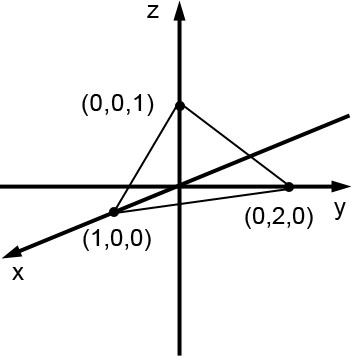
\includegraphics[width=0.35\textwidth]{TetExample.jpg}
  \end{center}
\end{figure}\\
Recall that the volume is the region under the plane $z = 1 - x - y/2$ and over  
\begin{align*}
  R = \{ (x,y) \ | \ 0 \le x \le 1- y/2, \ 0 \le y \le 2 \}.
\end{align*}
Because $z$ lies between 0 and $z = 1 - x - y/2$, the volume, $S$, can be described as
\begin{align*}
  S = \{ (x,y,z) \ | \ 0 \le x \le 1- y/2, \ 0 \le y \le 2, \ 0 \le z \le 1 - x - y/2 \}.
\end{align*}
The volume can be calculated with the triple integral
\begin{align*}
  \mathop{\int_{0}^{2} \! \int_0^{1-y/2} \int_0^{1-x-y/2} }dzdxdy
  &= \mathop{\int_{0}^{2} \! \int_0^{1-y/2}  } ( 1-x-y/2) dxdy\\
  &= \mathop{\int_{0}^{2}  } \Big( x-\frac{x^2}{2}-\frac{xy}{2}\Big)\Big|_0^{1-y/2} dy \\
  &= \mathop{\int_{0}^{2}  } \Big( (1-y/2)-\frac{(1-y/2)^2}{2}-\frac{(y-y^2/2)}{2}\Big) dy \\
  &= \mathop{\int_{0}^{2}  } \Big( 1 - \frac{y}{2}-\frac{1}{2} + \frac{y}{4} -\frac{y^2}{2}-\frac{y}{2}+\frac{y^2}{4}\Big) dy \\
  &= \mathop{\int_{0}^{2}  } \Big( \frac{1}{2} - \frac{y}{2}  -\frac{y^2}{4} \Big) dy \\
  &= \frac{2}{2} - \frac{4}{4}  -\frac{8}{12} \\
  &=  -\frac{3}{4}
\end{align*} 
Wrong!
% ~~~~~~~~~~~~~~~~~~~~~~~~~~~~~~~~~~~~~~~~~~~~~~~~~~~~~~~~~~~~~~~~~~~~~~~~~~~~~~~~~
\item % VOLUME OF AN ELLIPSOID
We are given the transformations
\begin{align*}
  x=au, \quad y=bv, \quad z=cw.
\end{align*}
The Jacobian becomes
\begin{align*}   J &=  
  \begin{vmatrix}
   \pxu &  \pxv \\ \\
   \pyu & \pyv \\
  \end{vmatrix}
  =     \begin{vmatrix}
 a&0&0\\
 0&b&0\\
 0&0&c\\
  \end{vmatrix}
  = abc.
 \end{align*}
 The solid enclosed by the ellipsoid is the image of the unit sphere $u^2 + v^2 + w^2 \le 1$. Using that a sphere has volume $\frac{4}{3} \pi r^3$, we find that 
\begin{align*}
  \iiint\limits_{V} dxdydz
  &=  \iiint\limits_{u^2+v^2+w^2 \le 1} abc \ dudvdw \\
  &=  abc \iiint\limits_{u^2+v^2+w^2 \le 1} \ dudvdw \\
  &=  abc (\text{volume of a sphere}) \\
  &=   \frac{4\pi abc}{3} 
\end{align*}
%% ~~~~~~~~~~~~~~~~~~~~~~~~~~~~~~~~~~~~~~~~~~~~~~~~~~~~~~~~~~~~~~~~~~~~~~~~~~~~~~~~~
%\item % BETA FUNCTION  KEEP?????
% We are given that 
% \begin{align*}
%  B(x,y) &= \int_0^1 t^{x-1}(1-t)^{y-1}dt.
%\end{align*}
% ~~~~~~~~~~~~~~~~~~~~~~~~~~~~~~~~~~~~~~~~~~~~~~~~~~~~~~~~~~~~~~~~~~~~~~~~~~~~~~~~~
\EEN % END OF SOLUTIONS

\end{document}

